\documentclass{standalone}
\usepackage{tikz}
\usetikzlibrary{shapes.geometric, arrows, positioning}


\begin{document}

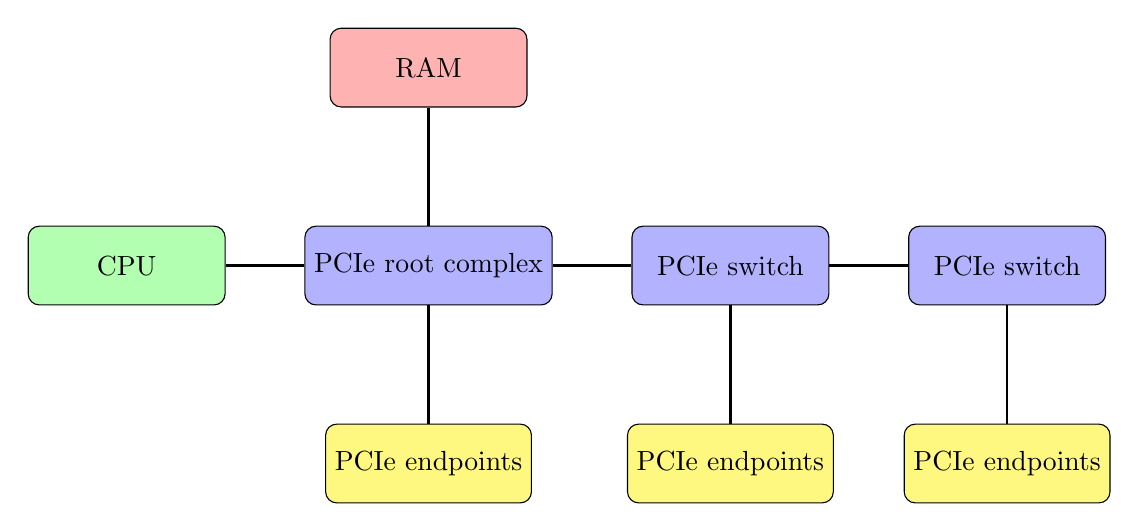
\begin{tikzpicture}[node distance=1.5cm and 1cm]

\tikzset{
    block/.style = {rectangle, rounded corners, minimum width=2.5cm, minimum height=1cm, text centered, draw=black, fill=blue!30},
    endpoint/.style = {rectangle, rounded corners, minimum width=2.5cm, minimum height=1cm, text centered, draw=black, fill=yellow!50},
    cpu/.style = {rectangle, rounded corners, minimum width=2.5cm, minimum height=1cm, text centered, draw=black, fill=green!30},
    ram/.style = {rectangle, rounded corners, minimum width=2.5cm, minimum height=1cm, text centered, draw=black, fill=red!30},
    arrow/.style = {thick,->,>=stealth}
}

% Nodes
% below right=\verdist and \hordist of conc
\node (cpu) [cpu] {CPU};
\node (root) [block, right=of cpu] {PCIe root complex};
\node (ram) [ram, above=of root] {RAM};

\node (switch1) [block, right=of root] {PCIe switch};
\node (endpoint1) [endpoint, below=of root] {PCIe endpoints};
\node (switch2) [block, right=of switch1] {PCIe switch};
\node (endpoint2) [endpoint, below=of switch1] {PCIe endpoints};
\node (endpoint3) [endpoint, below=of switch2] {PCIe endpoints};

% Connections
\draw [thick] (cpu) -- (root);
\draw [thick] (root) -- (ram);
\draw [thick] (root) -- (switch1);
\draw [thick] (switch1) -- (switch2);
\draw [thick] (root) -- (endpoint1);
\draw [thick] (switch1) -- (endpoint2);
\draw [thick] (switch2) -- (endpoint3);

\end{tikzpicture}

\end{document}

